\subsection{GUI}

The development of all graphic environments can be traced directly to
Ivan Sutherland's sketchpad. Its ideas \emph{still influence how every
  computer user thinks about computing.}\cite{graphics:sutherland__sketchpad}

\begin{wrapfigure}{r}{40mm}
  \begin{center}
    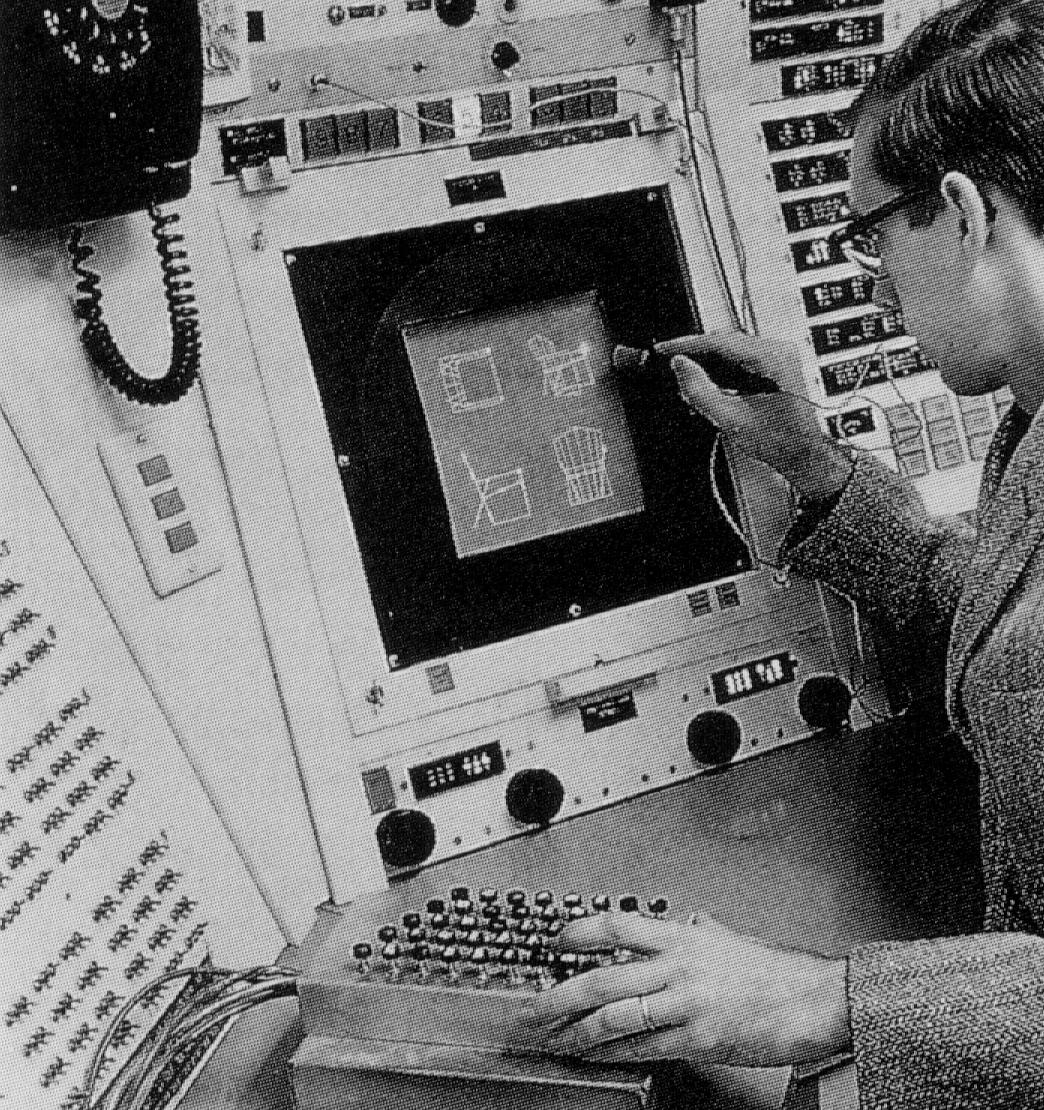
\includegraphics[scale=0.15]{images/sketchpad.jpeg}
  \end{center}
  \caption{Sketchpad console, circa 1962. \cite{hypertext:muller__vision_and_reality}}
\end{wrapfigure}

It did that by introducing graphic metaphors and devices, such as the
light-pen, the rubber band graphic manipulation, icons and a great
deal of the things most people take as ``natural'' when manipulating
modern GUI. \cite{graphics:sutherland__sketchpad}

But the major influence for programming paradigms was because its
object oriented features, which along with Simula \footnote{Both share
  a common ancestor in the work of Douglas T. Ross
  \cite{graphics:sutherland__sketchpad}} had a major impact in the
inspiration and development of Smalltalk: 

\begin{quote}
  What Simula was allocating were structures very much like the
  instances of Sketchpad. There were descriptions that acted like
  masters and they could create instances, each of which was an
  independent entity. What Sketchpad called masters and instances,
  Simula called activities and processes. ...

  This was the big hit, and I've not been the same since.
  \cite{smalltalk:kay_alan__early_history_smalltalk}
\end{quote} 
